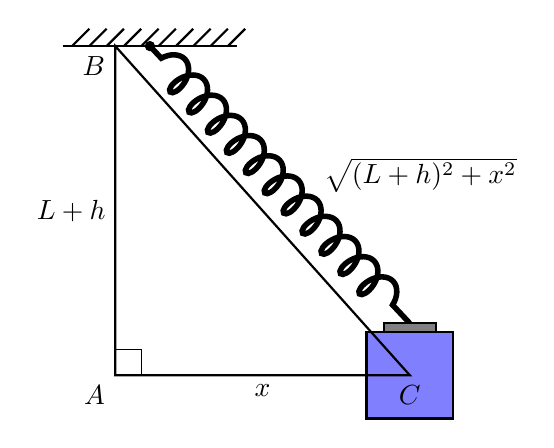
\begin{tikzpicture}[scale=1.1]
	\def\H{3}
	\def\X{3}
	\def\massw{1}
	\def\massh{1}
	\def\ceilw{1}
	\def\tip{Stealth[length=5pt, inset=2pt]}
	
	% Ceiling
	\draw[thick] (-\ceilw,\H+0.8) -- (\ceilw,\H+0.8);
	\foreach \x in {-0.9,-0.7,...,0.9}
	\draw[thick] (\x,\H+0.8) -- ++(0.2,0.2);
	
	% Fixed support
	\filldraw (0,\H+0.8) circle (1.5pt);
	
	% Dashed center line (upper only)
%	\draw[dashed] (0,\H+0.8) -- (0,0);
	
	% Mass block (upper connection only)
	\draw[fill=blue!50, thick]
	(\X-\massw/2, -\massh/2) rectangle 
	(\X+\massw/2, \massh/2);
	
%	\node at (\X,0) {$m$};
	
	% Top spring
	\draw[line width=2pt,
	decoration={
		coil,
		aspect=0.6,
		segment length=10pt,
		amplitude=6pt,
		pre length=6pt,
		post length=6pt
	},
	decorate]
	(0,\H+0.8) -- (\X,\massh/2 + 0.1);
	
	% Connector
	\draw[fill=gray, thick] (\X-0.3, \massh/2) rectangle (\X+0.3, \massh/2+0.1);
	
	% Horizontal displacement
%	\draw[blue!80, -\tip, thick]
%	(0,0) -- (\X-\massw/2,0);
	
%	\node[above] at (\X/2-\massw/4,0) {$x$};
	
	% Vertical label
%	\def\arrowh{0.2}
%	\draw[thick] (-0.7,\arrowh) -- (-0.3,\arrowh);
%	\draw[\tip-\tip] (-0.5,\H+0.8) -- (-0.5,\arrowh);
%	\node[left] at (-0.6,{\arrowh + (\H+0.8 - \arrowh) / 2}) {$L+h$};
	
	% Spring constant
%	\node at (2,2.4) {$k$};
	
	% Points
	\coordinate (A) at (-0.4,0);
	\coordinate (B) at (-0.4,\H+0.8);
	\coordinate (C) at (\X,0);
	
	% Triangle
	\draw[thick] (A) node[below left] {$A$} -- (B) node[below left] {$B$} -- (C) node[below] {$C$} -- cycle;
	
	% Right angle mark
	\draw (-0.4,0) rectangle (-0.1,0.3);
	
	% Labels
	\node[left] at (-0.4,\H/2 + 0.4) {$L+h$};
	\node[below] at (\X/2-0.2,0) {$x$};
	\node[above right] at (\X/2+0.4,\H/2+0.5) {$\sqrt{(L+h)^2 + x^2}$};
	
\end{tikzpicture}